\documentclass[10pt,
%handout
aspectratio=169
]{beamer}
\usepackage[utf8]{inputenc}
\usepackage[T1]{fontenc}
\usepackage{lmodern}

\usepackage{nicefrac}
\usepackage{braket}
\usepackage{booktabs}

%\usepackage[backend=biber,style=chem-acs]{biblatex}
%\bibliography{biblio}


\usetheme{metropolis}
\setbeamercolor{block title}{use=structure,fg=white,bg=structure.fg!75!black}
\setbeamercolor{block body}{parent=normal text,use=block title,bg=block title.bg!10!bg}


\usepackage{tikz}
\usetikzlibrary{positioning, decorations.markings, decorations.pathmorphing, calc}

\usepackage{siunitx}
\usepackage{mhchem}
\usepackage{minted}
\setminted{  
	frame=lines,  
	framesep=2mm,  
	baselinestretch=1.2,  
	fontsize=\footnotesize,  
	linenos,  
	breaklines,
	tabsize=2
}  

\author{Pierre Beaujean (\href{mailto:pierre.beaujean@unamur.be}{pierre.beaujean@unamur.be})}
\title{Advanced Python for advanced users}
\subtitle{... And a few concepts of computer science}
\institute{University of Namur}
\date{March 2025 (version of  \today)}

\allowdisplaybreaks

\begin{document}
\begin{frame}[plain]
	\maketitle
\end{frame}

\begin{frame}{Table of content}
	\tableofcontents
\end{frame}

\section{Back to basics}

\begin{frame}{Computer?}
	As far as you are concerned, a computer contains:\begin{itemize}
		\item A \textbf{CPU}, which execute (\textit{assembler}) code. Nowadays, there are also \textbf{GPUs} which can fulfill this role.
		\item Different kind of \textbf{memories} (cache, RAM, disk, etc), some of which can be addressed differently (\textit{e.g.}, through files).
		\item Some interfaces to the outside world, via peripherics (screen,  mouse, Ethernet, etc).
	\end{itemize}
	
	By itself, the CPU only moves bytes around in memory, and can perform operation on them. It understands the concept of \textbf{integers} and \textbf{floating point numbers} (IEEE-754 shenanigans), but that's about it. 
	
	Most functionalities of a computer (\textit{e.g.}, files) are in fact available thanks to the \textbf{operating system}, which offers, \textit{e.g.}, an unified interface to peripherics.
\end{frame}

\begin{frame}
	The \textbf{assembler} is a pretty simple (and CPU-dependent) language. For example, it does not understand the concept of strings (which explains why Fortran and C implements them differently). And, among other things, \textit{advanced} concepts like \textit{loops} are not directly available.
	
	 So... A meme will now ensue.
	
	\begin{center}
		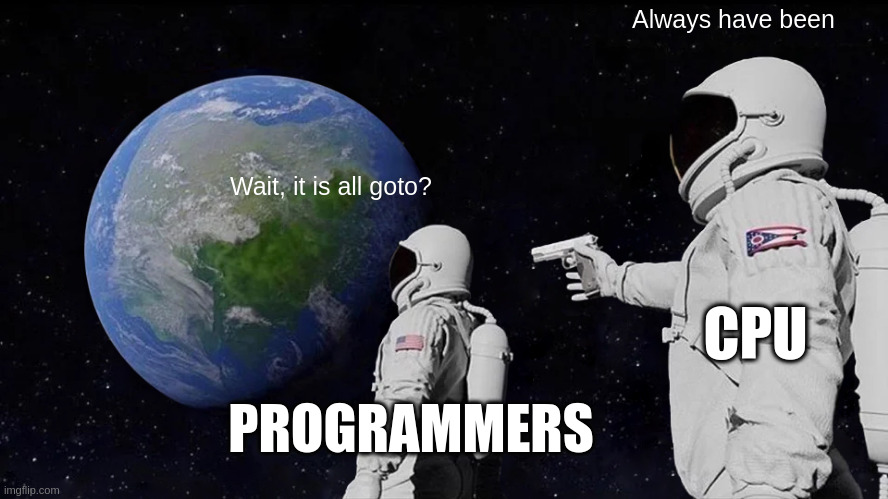
\includegraphics[width=.6\linewidth]{im/meme-goto}
		
		(Note: it is in fact \textbf{conditional jumps})
	\end{center}
\end{frame}

\begin{frame}{Programming in Python}
	A programming language enables you to express complex logic (\textit{e.g.}, loops, conditionals) in a structured and readable manner. This code is then either translated into machine instructions by a \textbf{compiler} or executed directly by an \textbf{interpreter}. While interpreted languages tend to be slower, they offer advantages such as dynamic execution (\mintinline{python}|exec()|), reflexivity (\mintinline{python}|getattr()|), and the ability to modify itself at runtime.
	
	Python is an \textbf{interpreted} language, but it is also \textit{just-in-time compiled} into an intermediate bytecode representation (stored in \mintinline{text}|__pycache__|). Over time, this process optimizes execution by reducing redundant checks, making subsequent runs of the code faster.
\end{frame}



\begin{frame}[fragile]
	The way to write the code is referred to as a \textbf{programming paradigm}, a relatively high-level way to conceptualize and structure the implementation of a computer program.\footnote{\url{https://en.wikipedia.org/wiki/Programming_paradigm}} Among others, there are:\begin{itemize}
		\item \textbf{Imperative}, in which the code directly controls execution flow and state change. This includes the famous \textbf{procedural} (\mintinline{text}|x = a(); y = b(x);|) and \textbf{object-oriented} (\mintinline{text}|x = X(); x.b();|) approaches.
		\item \textbf{Declarative}, in which code declares properties of the desired result, but not how to compute it, it describes what computation should be performed. This include the (in)famous \textbf{functional} approach (\mintinline{text}|(b(a()))|), but also programs based on \textbf{logic and constraints} (\mintinline{text}|x: int; y: int; x+y < 3;|).
		\item But also: \textbf{concurrent}, \textbf{visual}, etc...
	\end{itemize}
	
	To a certain extent, all paradigm can be used in all languages. Python is generally approached as an POO language.
	\vspace{1em}
\end{frame}

\begin{frame}{Note on the ``who''}
In the rest of this presentation, I will (sometimes) distinguish three kinds of people:\begin{enumerate}
	\item The \textbf{developers}, who actually develop the code/library and eventually provide an API (\textit{application programming interface}).
	\item The \textbf{programmers}, who use the API provided by the code/library and develop on top of it.
	\item The \textbf{users}, who use the program/executable, but do not program.
\end{enumerate}
\end{frame}

\section{It's all about abstraction}

\begin{frame}{Abstractions}
	A well-designed program should be \textbf{modular}, with each module having clear and specific responsibilities. They can then work together . One of the best ways to achieve this is through \textbf{abstraction}, which means focusing on what matters while ignoring unnecessary details. There are several levels of abstraction:
	\begin{enumerate}
		\item \textbf{Abstraction by Parameterization}: Use parameters instead of hard-coded values to make code flexible and reusable.
		\item \textbf{Abstraction by Procedures}: Structure your code using functions that call one another, rather than relying on \textit{copy-paste-modify} patterns.
		\item \textbf{Abstraction by Specification}: Describe \textbf{what} the code should do, not \textbf{how} it does it. This allows you to change the implementation without affecting other parts of the program. (More on this later.)
		\item \textbf{Data Abstraction}: Instead of using raw data, encapsulate it in \textbf{abstract data types} (e.g., objects). Type hierarchies using \textbf{inheritance}, with child classes inheriting behaviors from parent classes. (More on this later.)
		\item And others: syntaxic sugar, etc.
	\end{enumerate}
\end{frame}

\begin{frame}[fragile]
	Example(s):
	\begin{minted}{python}
# without any abstraction
print('perimeter of circle is', 2 * 3.141592 * 3.5)
print('area is', 3.141592 * 3.5 ** 2)
# abstraction by parameterization
from math import pi as PI

r = 3.5
print('perimeter of circle is', 2 * PI * r)
print('area is', PI * r ** 2)
# abstraction by procedure
def info_circle(r: float) -> None:
	print('perimeter of circle is', 2 * PI * r)
	print('area is', PI * r ** 2)

info_circle(3.5)
info_circle(7.2)
\end{minted}
\end{frame}


\begin{frame}[fragile]
	An example of data abstraction (\texttt{fp32}):
	\begin{center}
		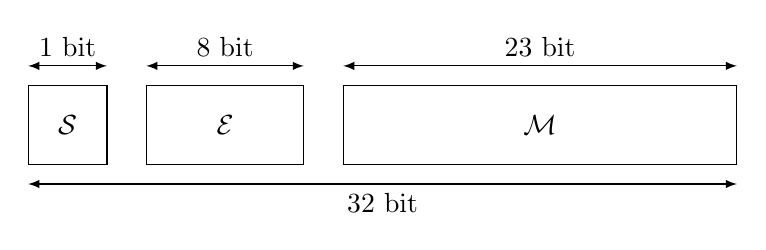
\begin{tikzpicture}
			\draw (0, 0) rectangle +(1, 1)  node[midway] {$\mathcal{S}$};
			\draw (1.5, 0) rectangle +(2, 1)  node[midway] {$\mathcal{E}$};;
			\draw (4, 0) rectangle +(5, 1)  node[midway] {$\mathcal{M}$};
			\draw[latex-latex] (0,1.25) -- +(1,0) node[midway,above]{1 bit};
			\draw[latex-latex] (1.5,1.25) -- +(2,0) node[midway,above]{8 bit};
			\draw[latex-latex] (4,1.25) -- +(5,0) node[midway,above]{23 bit};
			\draw[latex-latex] (0,-.25) -- +(9,0) node[midway,below]{32 bit};
		\end{tikzpicture}
		\begin{equation*}
			x = (-1)^\mathcal{S} \times 2^{\mathcal{E}-2^7} \times \left(1+\frac{\mathcal M}{2^{23}}\right).
		\end{equation*}
	\end{center}
	And yet...
	\begin{minted}{python}
# let's play with floats:
x = 2.5e7  # S=0, E=151, M=4111392
y = x - 3.25e-2
	\end{minted}
	This is a powerful abstraction!
\end{frame}

\section{Abstraction by specification}

\begin{frame}{Design by contract (i.e., abstraction by specification)}
	\vspace*{1em}
	\begin{columns}
	\column{.5\linewidth}
	\parskip=1em
	The ``design by contract" approach prescribes that developers should define formal(?), precise(?) and verifiable(?) interface \textbf{specifications} for software components (functions, classes, modules, programs, etc). 
	
	The ``contract'' is the following: $\{P\land I\} \,\underline{S}\,\{Q\land I\}$ ($\land$ side effects). Generally, $\lnot (P \land I)\implies \text{errors}$, but it is not necessarily true in all cases (and it does not have to be). 
	
	\textbf{Notice that this does not say what is $\underline{S}$.} This is thus mostly useful for the programmer (and the user).
	
	\column{.5\linewidth}
	\begin{center}
		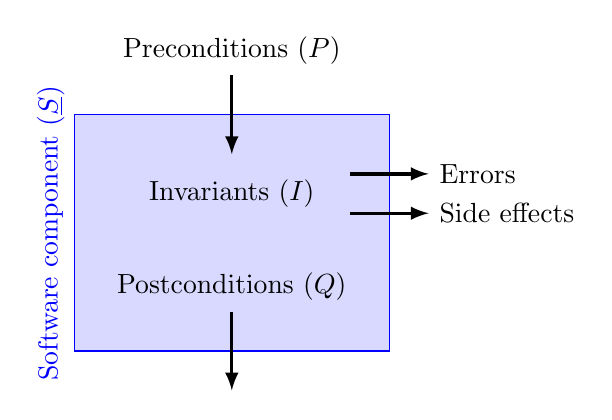
\begin{tikzpicture}
			\draw[blue,fill=blue!15] (0, 0) rectangle +(4, 3);
			\draw[blue]  (0, -.5) node[anchor=south west,rotate=90]{Software component ($\underline{S}$)};
			\draw[-latex,very thick] (2, 3.5) node[above]{Preconditions ($P$)}-- +(0, -1);
			\draw[-latex,very thick] (2, 0.5) node[above]{Postconditions  ($Q$)}-- +(0, -1);
			\draw[-latex,very thick] (3.5, 2.25) -- +(1, 0) node[right]{Errors};
			\draw[-latex,very thick] (3.5, 1.75) -- +(1, 0) node[right]{Side effects};
			\draw (2, 2) node{Invariants ($I$)};
		\end{tikzpicture}
	\end{center}
	\vspace*{1em}
	+ Eventual performances guarantees.
	\end{columns}
\end{frame}

\begin{frame}
	\vspace*{1em}
	\begin{columns}
		\column{.5\linewidth}
		\begin{itemize}
			\item The \textbf{preconditions} are predicates that must be true before the execution of the component (it generally boils down to the type of the inputs and their respective domains). It must be guaranteed by \textbf{the caller}. If a precondition is violated, the effect becomes undefined.
			\item The \textbf{postconditions} are predicates that must be true after execution (if the preconditions are true), which is guaranteed by the \textbf{callee}.
			\item The \textbf{invariants} are predicates that must be true before and after execution. This is guaranteed by the caller \textbf{and} the callee (but mostly the later).
		\end{itemize}
		
		\column{.4\linewidth}
		\begin{center}
			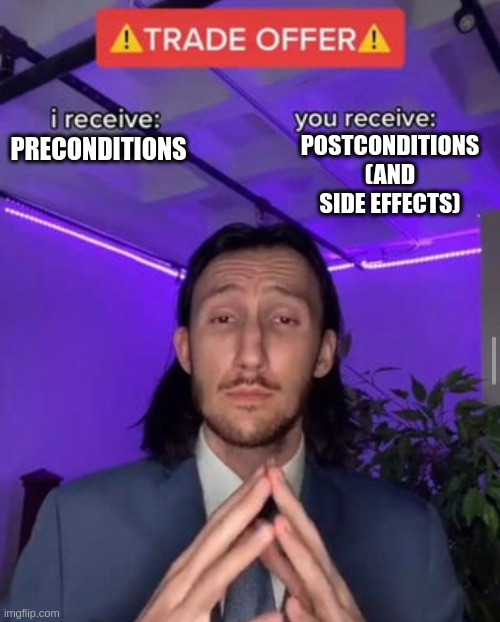
\includegraphics[width=\linewidth]{im/meme-prepost}
		\end{center}
	\end{columns}
\end{frame}

\begin{frame}[fragile]
	Example: $P \equiv x\in\mathbb{R}$ (not necessarily true in python!), $Q\equiv \mathcal{R} = |x|$, $I \equiv \text{yes}$, $\underline{S} \equiv$\begin{minted}{python}
def _abs(x: float) -> float:
	return -x if x < 0 else x  # note: that's called syntaxic sugar
	\end{minted}
	Here, $sp(\underline{S}, P \land I) \implies Q \land I$, so this program is valid. Indeed, \begin{align*}
		Q' &= sp(\text{\mintinline{python}|return -x if x < 0 else x|}, x\in\mathbb{R}) \\
		&= (\mathcal{R} = -x \land x < 0 \land x\in\mathbb{R}) \lor (\mathcal{R} = x \land x \geq 0 \land x\in\mathbb{R})\\
		&= [(\mathcal{R} = -x \land x < 0) \lor (\mathcal{R} = x \land x \geq 0)]  \land x\in\mathbb{R}
	\end{align*}
	and $Q' \implies Q \land I$. Note that \mintinline{python}|_abs("test")| is indeed undefined.
	
	This is how you should ensure that your programs are valid, except nobody does that in practice (except in security contexts, like planes, trains, or in space). Note that one of the implicit assumption is that the interpreter works correctly (so you also need to ``prove" the interpreter if you want to be 100\% correct).
\end{frame}

\begin{frame}
	\begin{itemize}
		\item \textbf{Errors:} we will see below how to play with errors, but if one sticks to \textit{design by contract} alone, this is not required, since the preconditions \textbf{must always} be fulfilled. 
		
		In practice, it is generally not the case (\textit{never trust user input}!), and having undefined behaviors may lead to unexpected bugs (since the execution can continue) or even security issues. Thus, one can abide to \textbf{defensive programming} instead, which consists in weakening the precondition (or delete it), and either report failure (throwing exceptions) or running in degraded mode.\footnote{Purely falling would be a bit annoying in a plane ;)}
		 \item This leads to \textbf{side-effects}, which is the fact that the code have an observable effect other than reading its input and giving an output. Other example of side-effects include: performing I/O, modifying a non-local variable (\textit{e.g.}, matplotlib's \mintinline{python}|pyplot| interface, which is a state machine), or mutate an argument (\textit{e.g.}, sorting a list in-place).\footnote{BLAS and LAPACK are customary of such practices.} \textbf{All} such side-effects should be \textbf{properly} documented.
	\end{itemize}
\end{frame}

\begin{frame}
	In practice, be nice to your programmers/users (... and to future you, for that matter) that your \textbf{specifications} contains the following:\begin{itemize}
		\item Document your inputs, it is better than nothing. This include their types (in some language, it is in the definitions) and their \textbf{domain} (\textit{e.g.}, for \mintinline{python}|sqrt(x)|, \mintinline{python}|x >= 0|).
		\item Document the \textbf{effect} of the code rather than what it does (which does not prevent you to have another document which details the algorithms).
		\item If possible, document all \textbf{side effects}, in particular if you mutate an argument.
	\end{itemize}
	
	Since you will probably never properly prove your pre/postconditions, you don't have to use a mathematical language to express everything.\footnote{personally, I write my pre/post-conditions using the programming language itself, for example \mintinline{python}|x >= 0 and 0 <= y < 3 and z in ['a', 'b', 'c']|.} Even if any spoken language is ambiguous, a nice textual description is better than nothing.
	
	The goal is therefore to provide a ``framework" for things you should document, rather than a set of rules.
\end{frame}

\begin{frame}
	Caution:
\begin{center}
	{\LARGE \textit{Programming by contract} assume that \textbf{everyone} write, read, understand, and follow the specifications.}
\end{center}
That's rarely the case in amateur projects (including some of mine, by the way).
\end{frame}

\begin{frame}{Documentation(s?)}
	\begin{itemize}
		\item The documentation is therefore the place where you indicate your pre/post-conditions, side effects, etc. Note that these concepts applies to any component you can think of (even a CLI program has inputs and outputs), although with different names. Again, ``framework'' rather than set of rules.
		\item Be nice to your programmers/users: details the installation procedure as much as possible (detail the dependencies if any), provide examples,\footnote{... But an example alone is not a good documentation, thought.} etc. We all have in mind good and bad documentation... Let's not be an example of the latter ;)
		\item There is no convention for the form of your documentation (it can be done with any tool you want), but it is generally better to diminish the amount of manual work, which means that documentation \textbf{auto-generation} is a good idea.
	\end{itemize}
\end{frame}

\begin{frame}[fragile]
	The idea of auto-generation is to write a part of your documentation directly in the code as comments, then to use a tool that read such comments  and generate a nice document (generally a set of HTML pages) as output. 
	
	The tool of the trade here is generally Doxygen (see \url{https://www.doxygen.nl/}), which was first created for C++:
	\begin{minted}{cpp}
class Dog {
	public:
	/**
	* \brief Creates a new Dog.
	*
	* Creates a new Dog named `_name`.
	*
	* \param _name The dog's name.
	*/
	Dog(const char* _name);
};
	\end{minted}
	... But works for many languages (including Python and Fortran).
\end{frame}

\begin{frame}
	But in Python, nobody  agrees yet.\footnote{Sphinx seems to win for major projects, thought.} There are three concurrent documentation formats (ReST, numpy, and Google) and a plethora of tools to interpret them, among which:\begin{itemize}
		\item Doxygen, which has its own format ;
		\item autodoc (used with Sphinx), which requires to write in ReST (more complete than markdown, but more complex) ;
		\item mkdocstring (used with mkdocs), which uses markdown ;
		\item pdoc3, which uses markdown.
	\end{itemize}
	All three of four generates an HTML output (which is generally what you want). They supports LaTeX formula by various means.
\end{frame}

\begin{frame}
	\begin{center}
		{\LARGE DEMO TIME!}
	\end{center}
	
	\begin{itemize}
		\item Sphinx
		\item \mintinline{bash}|python -m doctest -v neighbour_search/*.py|
	\end{itemize}
\end{frame}
\begin{frame}{Error handling (\textit{exceptions})}
As mentioned above, there are two possible reasons for reporting an error:\begin{enumerate}
	\item When the precondition is not fulfilled. Again, you should normally not check that, and thus, not report an error for that. However... This is still useful for the developer during implementation. Thus, \textbf{if checking (a part of) the precondition is cheap},\footnote{$\mathcal{O}(1)$, no more.} you can use \mintinline{python}|assert|, which is a function/statement available in many languages that is only compiled/interpreted in ``debug'' mode.\footnote{calling \texttt{python -O -c "assert false"} results in no error.}
	\item When you want to avoid undefined behavior by weakening the preconditions and issuing errors instead.
\end{enumerate}
\end{frame}

\begin{frame}[fragile]
And there are two ways to report an error. One is to use the return value or mutate a global variable (or, on languages that allows it, mutate an input designated for that, like \texttt{ierror}):\begin{minted}{python}
	def normalize(x: np.ndarray) -> int:
	"""
	pre: x is a vector
	post: if return value is 0, x is normalized, if return value is 1, it is not.
	"""
	norm = np.linalg.norm(x)
	if norm == 0:
	return 1
	x /= norm
	return 0
\end{minted}
Although totally fine, this is a bit long. Also, the caller can ignore the return value,\footnote{Many bugs in old AND modern programs are due to non-checked return values when allocating memory.} which would in practice create an undefined behavior.
\vspace{1em}
\end{frame}

\begin{frame}
This is why many ``modern'' programming languages propose a mechanism called \textbf{exceptions}.  It works like this:\begin{itemize}
	\item When an issue should be issued, the code \textbf{throw} an exception (which can be an integer, a string, or something more complex like and object which allows to provide context).
	\item The execution propagate up in the call stack, to a point where the error can be handled. If there is none, the execution terminates badly.
\end{itemize}
This force the caller to handle the exception. It also effectively separate the code that detect the error and the one that handles it.
\end{frame}

\begin{frame}
\begin{center}
	{\LARGE DEMO TIME!}
\end{center}
\end{frame}

\begin{frame}
The take home message here is:\begin{itemize}
	\item \mintinline{python}|assert| for the developers,
	\item \mintinline{python}|throw| (+ documentation) for the programmers, and
	\item a nice error message (eventually in \texttt{stderr}) for the users. The stacktrace frighten them.
\end{itemize}


And, by the way...

\begin{center}
	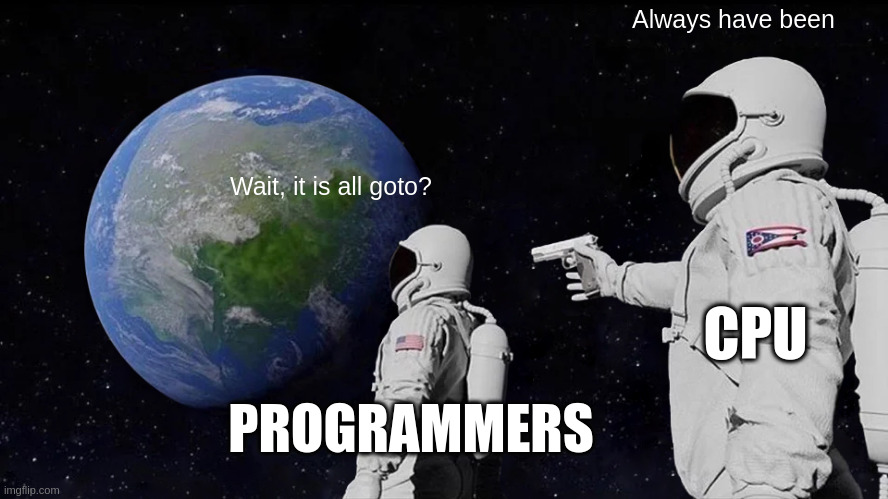
\includegraphics[width=.5\linewidth]{im/meme-goto}
\end{center}
\end{frame}

\begin{frame}{Testing}
	\begin{columns}
		\column{.5\linewidth}
		
		Per Wikipedia, ``software testing is the act of checking whether software satisfies expectations". 
		\parskip=1em
		
		It is \textbf{very} important, since it provides ways to check whether your code do what it is supposed to do without proving your code... Which does not guarantee that your code is correct, just that it seems to work under certain conditions, which is already something ;)
		
		\column{.5\linewidth}
	
	\begin{center}
		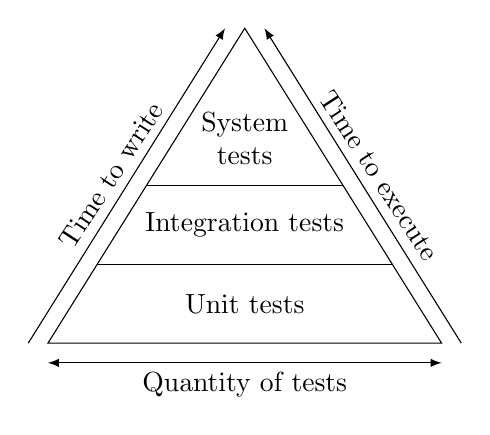
\begin{tikzpicture}
			\draw (0,0) -- +(5, 0) -- +(2.5, 4) --cycle;
			\draw[latex-latex] (0,-.25) -- +(5, 0) node[midway,below]{Quantity of tests};
			\draw[-latex] (-.25,0) -- +(2.5, 4) node[midway,above, rotate=57]{Time to write};
			\draw[-latex] (5.25,0) -- +(-2.5, 4) node[midway,above, rotate=-57]{Time to execute};
			
			\draw (2.5,.5) node{Unit tests};
			\draw (.62, 1) -- +(3.75,0);
			\draw (2.5,1.5) node{Integration tests};
			\draw (1.25, 2) -- +(2.5,0);
			\draw (2.5, 2.6) node[text centered, text width=1.25cm]{System tests};
		\end{tikzpicture}
		\parskip=1em
		
		(other kind of tests exists)
	\end{center}
\end{columns}
\end{frame}

\begin{frame}
	\begin{itemize}
		\item \textbf{Unit tests}: they test small parts of your code (\textit{i.e.}, a function or a class) and check its behavior. They are quick to run, and are written with the actual implementation in mind (white box testing) and maximize \textbf{coverage} (\textit{i.e.}, most if not all execution paths are checked). In some case, they go beyond checking that the pre/postconditions are true.\footnote{The pre/postconditions can be weaker than the actual implementation.} They generally use mock data.
		\item \textbf{Integration tests}: checks that the functions, classes, modules, etc of your project works together. They are higher level, and are not written with implementation in mind, only the specifications (black box testing). They generally use mock data or very simple real ones (think water in HF/STO-3G to check Mulliken charges).
		\item \textbf{System tests} (also called functional tests): high-level tests (to check that everything works together) with real data from real life. They generally check that the front-end program/library meets its requirements (think real medium-sized molecule, with a realistic method and basis set). They are generally manually launched!
	\end{itemize}
	All these constitute your \textbf{tests suite}.
\end{frame}

\begin{frame}
	Ideally, tests should: \begin{itemize}
		\item Be written as soon as possible. In fact, if you already have the specifications, you can start by writing (unit) tests that check those specifications before even writing the implementation. This is \textbf{test-driven development}. 
		\item Run often. A good practice is to have a \textbf{continuous integration (CI) pipeline}, which generally boils down to a script that runs all your unit and integration tests, automatically launched at every occasion (commit, PR, etc). This helps you to prevent \textbf{regressions}.
		\item Fail quickly. If you have to wait 20 minutes to know if your implementation fails, that's painful. This is why most tools allow you to run only one part of your test suite locally (and this is why \textbf{mock data} are useful).
		\item Be smart: no need to test EVERY input, only a few well-chosen ones ;)
		\item Test as much as possible, but not too much: no need to test that a dependency that you use works as intended, that's their job not yours!
	\end{itemize}
\end{frame}

\begin{frame}
	Speaking of mock data... Yet another \textit{``grimmerie"}:
	\begin{center}
	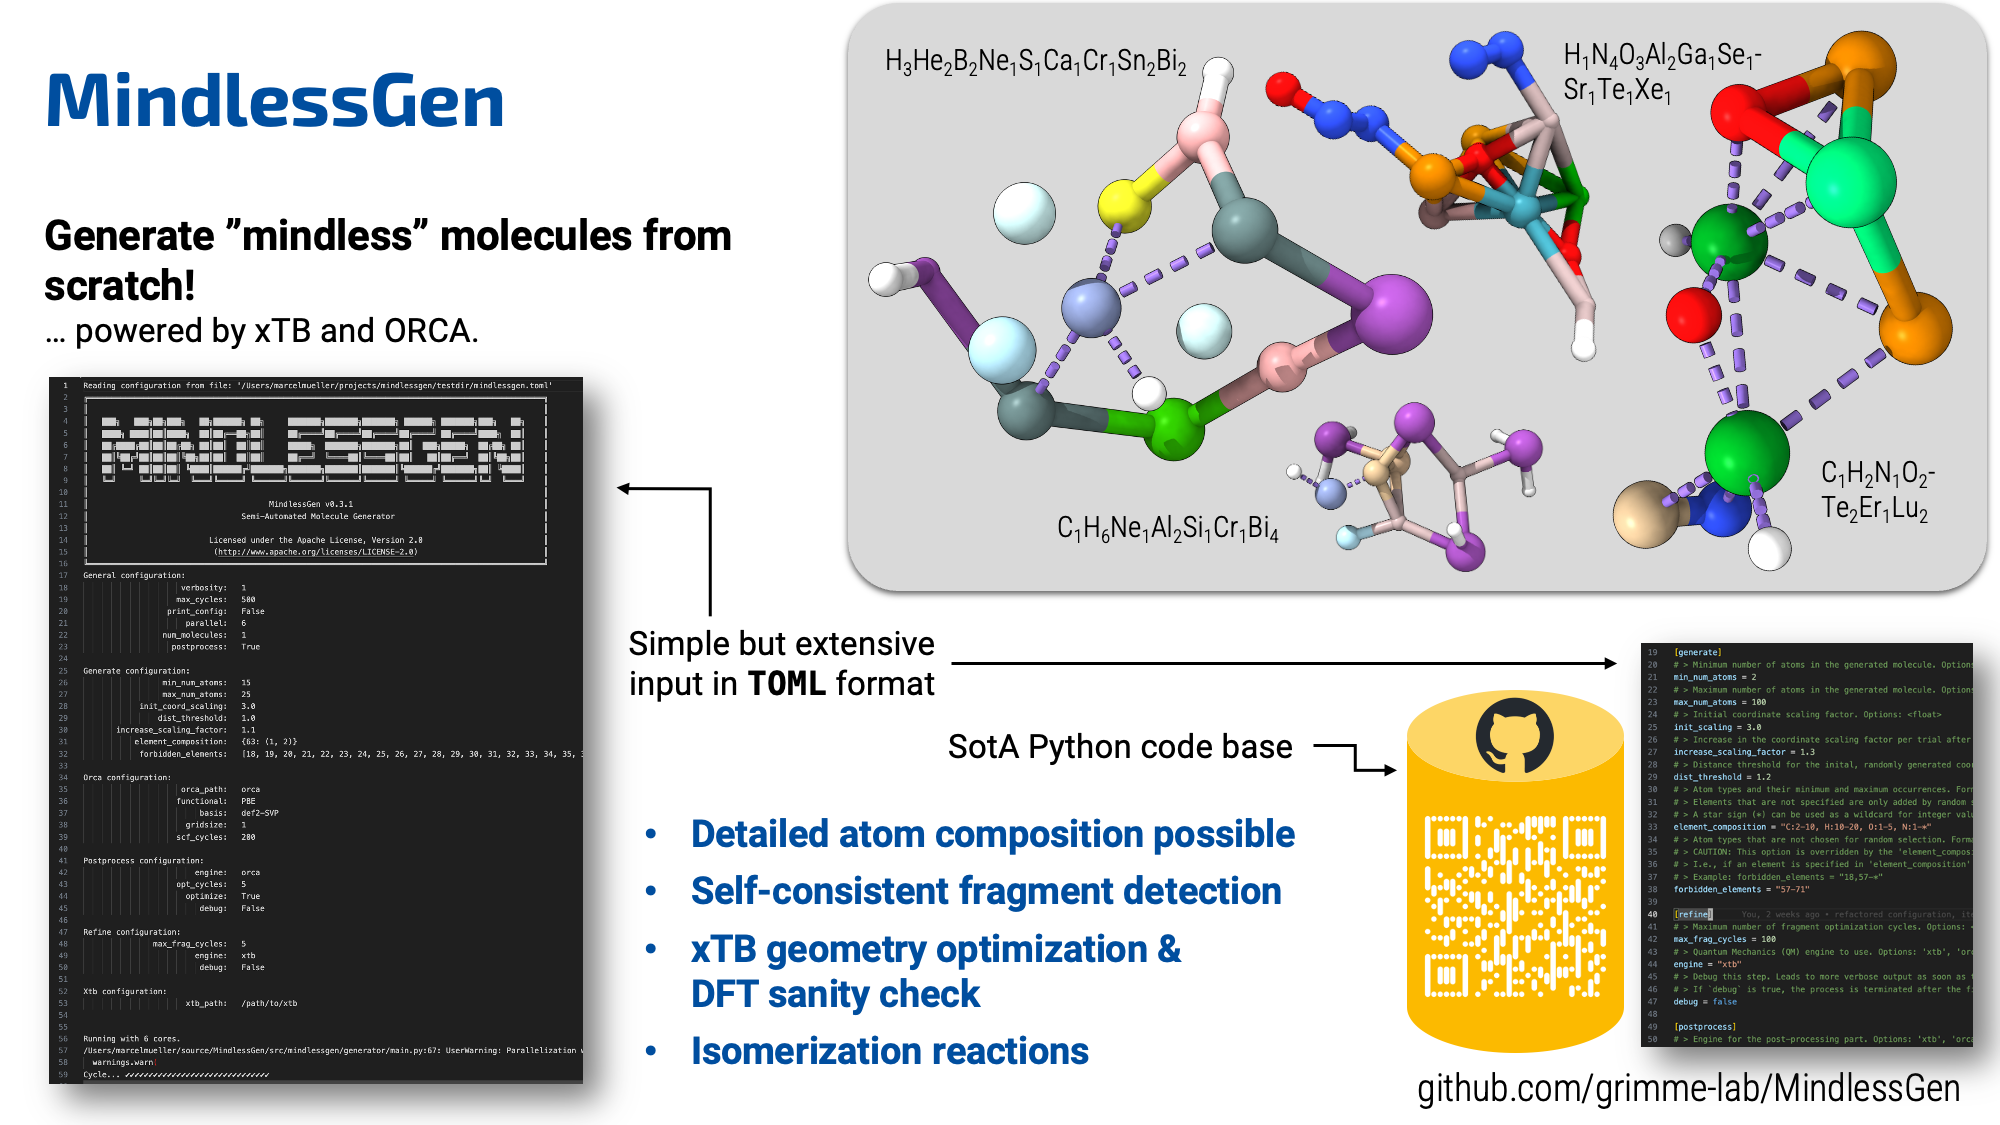
\includegraphics[width=.7\linewidth]{im/MindlessGen}
	\url{https://github.com/grimme-lab/MindlessGen/}
	\end{center}
\end{frame}

\begin{frame}
	How to write tests:\begin{itemize}
		\item Follow the following structure:\begin{enumerate}
			\item Setup: prepare any data you need for your test ;
			\item Stimuli: run the piece of code you want to test ;
			\item Verify: check that the output matches what you expect ;
			\item Teardown: clean up your mess, if any.
		\end{enumerate}
		In general, the first and last steps are common to many tests (\textit{e.g.}, the starting geometry of water is the same for an energy or optimization calculation).
		\item Separate your tests from your code: you may want to ship your library/program without its tests for actual use.
		\item Use a proper test framework! In python, this means either \texttt{unittest} or \texttt{pytest}, which both provide ways to call your test suite (or some parts of it) smoothly.
	\end{itemize}
\end{frame}

\begin{frame}
\begin{center}
	{\LARGE DEMO TIME!}
	
	\begin{itemize}
		\item \mintinline{python}|pytest| basics (create and run)
		\item fixtures
	\end{itemize}
\end{center}
\end{frame}

\section{Data abstraction}


\newcommand{\Ox}[1]{\ensuremath{\mathcal{O}(#1)}}

\begin{frame}{Data structures}
The idea behind common data structures (list, arrays, dictionary, sets, etc) is to provide efficient ways to store and retrieve data depending on the problem you want to solve.

To measure the efficiency, one measures the \textbf{computational complexity} of different tasks, defined as:\begin{equation*}
	T(n) = \mathcal{O}(g(n))  \text{ as } n\to\infty \implies \exists M, n_0\in\mathbb{N}^+: \forall n\geq n_0: |T(n)| \leq M |g(n)|,
\end{equation*}
where $T(n)$ is the function that measure the execution time of a given piece of code (generally a function) given an input of size $n$. In a sense, the big-$\mathcal{O}$ refers to the asymptotic behavior of $T(n)$ (and is thus also found when speaking about finite series). 

$g(n)$ is generally taken as simple as possible, such as $1$, $\log_2 n$ (generally written $\log n$), $n$, etc.
\end{frame}


\begin{frame}[fragile]
	Example:\begin{minted}{python}
def find1(a: list[int], v: int) -> int:
	"""
	Get the position of `v` in `a`.
	
	pre: `a` is a list of integers, `v` is an integer.
	post: if it exists in `a`, the index of `v` is returned if in `a`. A negative value is returned otherwise.
	"""
	for i in range(len(a)): 
		if a[i] == v:
			return i 
	return -1   # note: postcondition is less strict than actual implementation
	\end{minted}
In the worst case scenario (\mintinline{python}|v| is not in \mintinline{python}|a|), the loop is executed $n$ times, where $n$ is the size of \mintinline{python}|a|. This algorithm is thus $\Ox n$.
\end{frame}

\begin{frame}[fragile]
\begin{minted}{python}
def find2(a: list[int], v: int) -> int:
	"""
	Get the position of `v` in `a`.
	
	pre: `a` is a **sorted** list of integers, `v` is an integer.
	post: if it exists in `a`, the index of `v` is returned if in `a`. A negative value is returned otherwise.
	"""
	b, e = 0, len(a) - 1
	while e >= b:  # note: T(n) = 1 + T(n/2)
		p = (e + b) // 2  # note: integer division
		if a[p] == v:
			return p
		elif a[p] > v:
			e = p - 1    # then it's left
		else:
			b = p + 1   # then it's right
	return -1
\end{minted}
In the worst case scenario, the loop is executed $\log_2 n$ times, so $\Ox{\log n}$.
\end{frame}

\begin{frame}
	In a nutshell:
	\begin{table}
		\scriptsize
		\begin{tabular}{l cccc c cccc}
			\toprule
			Data & \multicolumn{4}{c}{Average time complexity} & & \multicolumn{4}{c}{Worst time complexity} \\
			\cline{2-5} \cline{7-10}
			structure& Access & Search & Insert & Delete && Access & Search & Insert & Delete \\
			\midrule
			Array & \textcolor{green}{\Ox 1} & \textcolor{red}{\Ox n} & \textcolor{red}{\Ox n} & \textcolor{red}{\Ox n} && \textcolor{green}{\Ox 1} & \textcolor{red}{\Ox n} & \textcolor{red}{\Ox n} & \textcolor{red}{\Ox n} \\
			List & \textcolor{red}{\Ox n} & \textcolor{red}{\Ox n} & \textcolor{green}{\Ox 1}  &\textcolor{green}{\Ox 1} && \textcolor{red}{\Ox n} & \textcolor{red}{\Ox n} & \textcolor{green}{\Ox 1}  &\textcolor{green}{\Ox 1}\\
			BS-tree &  \textcolor{orange}{\Ox{\log n}}  &  \textcolor{orange}{\Ox{\log n}}  &  \textcolor{orange}{\Ox{\log n}}  &  \textcolor{orange}{\Ox{\log n}}  && \textcolor{red}{\Ox n} & \textcolor{red}{\Ox n} & \textcolor{red}{\Ox n} & \textcolor{red}{\Ox n} \\
			(R)B-tree &  \textcolor{orange}{\Ox{\log n}}  &  \textcolor{orange}{\Ox{\log n}}  &  \textcolor{orange}{\Ox{\log n}}  &  \textcolor{orange}{\Ox{\log n}}  &  &  \textcolor{orange}{\Ox{\log n}}   &  \textcolor{orange}{\Ox{\log n}}  &  \textcolor{orange}{\Ox{\log n}}  & 
	 \textcolor{orange}{\Ox{\log n}}\\
	 Hash Table & --- & \textcolor{green}{\Ox 1} & \textcolor{green}{\Ox 1} & \textcolor{green}{\Ox 1} && --- & \textcolor{red}{\Ox n} & \textcolor{red}{\Ox n} & \textcolor{red}{\Ox n} \\
	 \bottomrule
		\end{tabular}
		\caption{Data structure operation costs, from \url{https://www.bigocheatsheet.com/}.}
	\end{table}
	Notes:\begin{itemize}
		\item In practice, nobody care how its implemented.
		\item All these structure have $\mathcal{O}(n)$ space complexity.
		\item Stack, Queue, List, etc are generally implemented as singly/doubled linked lists.
		\item Hash tables (dictionary) are generally a combination of an array (for which the hash function give the key) and some sort of list or tree to solve collisions.
		\item The \mintinline{python}|set| (and \mintinline{python}|frozenset|?) is implemented as a hash table.
		\item See below for BS (binary search) tree.
	\end{itemize}
\end{frame}
 
 \begin{frame}[fragile]{Oriented object programming (OOP)}
 	
 	The goal of OOP is to define new \textbf{abstract data types} (ADT), \textit{i.e.}, separate the concrete representation of the data and their (abstract) signification. For example, a \textit{molecule} (not that you should not define members like this):\begin{columns}
 		\column[t]{.25\linewidth}
 		\begin{minted}{python}
class Atom:
  symbol: str
  coordinates: list[float]
 	
class Molecule:
  atoms: list[Atom]
 		\end{minted}
 		\column[t]{.25\linewidth}
 		\begin{minted}{python}
class Molecule:
	symbols: list[str]
	positions: np.ndarray
 		\end{minted}
 		\column[t]{.25\linewidth}
\begin{minted}{python}
class Atom:
	symbol: str
	coordinates: list[float]

class Molecule:
	atoms: SearchTree[Atom]
\end{minted}
 	\end{columns}
In all three cases, although the \textbf{internal representation} (irep) of the molecule change, its behavior should not! And the programmer should not knwow  (or care) about what is inside.
 \end{frame}
 
\begin{frame}
	So, what do you need to do OOP?\begin{itemize}
		\item The \textbf{need} for an ADT (it is more frequent than you think!).
		\item An (abstract) \textbf{specification}: what your ADT is suppose to do? (again, focus on ``what'', not ``how''). This may include an \textbf{ADT invariant} (AI), something that should be true during the lifetime of an instance of the ADT.
		\item \textbf{The specification the methods}: these methods provides ways to interact with your ADT: normally, the programmer should never directly interact with your irep.\footnote{This is called \textbf{encapsulation}. Python is rather permissive here.} Furthemore,  no method should break the AI! 
		\item \textbf{An irep}: it should be chosen so that it allow you to  implements all specified methods. A useful tool in there is the definition of a \textbf{representation invariant} (RI), which translates the ADT invariant in concrete code. 
	\end{itemize}
	In python (and in other languages), an ADT is implemented via a \mintinline{python}|class|. Then, in the rest of the code, you \textbf{instanciate} your ADT and interact with these instances with the methods that where defined in the \mintinline{python}|class|.
	\vspace{1em}
\end{frame}

\begin{frame}
	\vspace{1em}
	\begin{columns}
	\column{.6\linewidth}
	(textbook) example: a \textbf{binary search (BS) tree}:\begin{itemize}
		\item The \textbf{need}: yes. Data are automatically sorted as a result!
		\item An (abstract) \textbf{specification}:  a binary search tree is a tree that allow binary search for fast lookup, addition, and removal of data items (here, integers). Each node of the tree has (at most) two children, the \textit{left} and the \textit{right}. The AI  is the following: ``each node is greater than all the ones in its left subtree and less than the ones in its right subtree''.
		\item \textbf{The specification the methods}: one needs at least \mintinline{python}|insert(k: int)|, \mintinline{python}|delete(k: int)|,  and \mintinline{python}|search(k: int)|.
		\item \textbf{An irep}: linked lists would do, but funny implementations exists with arrays.
	\end{itemize}
	\column{.4\linewidth}
	\begin{center}
		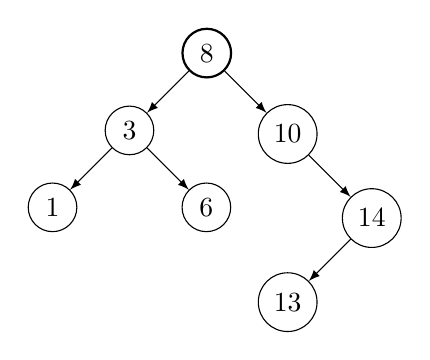
\begin{tikzpicture}[node distance=.75cm]
			\node[circle,draw,thick] (r8) {8};
			\node[circle,draw,below left=of r8] (r3) {3};
			\node[circle,draw,below right=of r8] (r10) {10};
			\node[circle,draw,below right=of r10] (r14) {14};
			\node[circle,draw,below left=of r14] (r13) {13};
			\node[circle,draw,below left=of r3] (r1) {1};
			\node[circle,draw,below right=of r3] (r6) {6};
			\draw[-latex] (r8) -- (r10);
			\draw[-latex] (r8) -- (r3);
			\draw[-latex] (r3) -- (r6);
			\draw[-latex] (r3) -- (r1);
			\draw[-latex] (r10) -- (r14);
			\draw[-latex] (r14) -- (r13);
		\end{tikzpicture}
	\end{center}
	Questions: how to perform:\begin{enumerate}
		\item \mintinline{python}|search(6)|, or
		\item \mintinline{python}|insert(12)|, or
		\item \mintinline{python}|delete(8)|,
	\end{enumerate}
	in order to keep the AI valid? And in the second case, what is the complexity?
\end{columns}
\end{frame}

\begin{frame}
	Useful methods:\begin{itemize}
		\item \textbf{Creators} (including, but not limited to, \textit{constructors}): allow to create instances of your ADT out of nowhere.
		\item \textbf{Producers}: create new instance from existing one(s). Particularly useful for \textbf{immutable} ADT, but you need to take care of the copy of your irep.\footnote{Shallow versus deep copy.}
		\item \textbf{Modifiers} (also called \textit{setters}): modifies the instance directly.
		\item \textbf{Observers} (also called \textit{getters}): provide access to properties of the instance.
	\end{itemize}
	A similar nomenclature is CRUD (create, read, update, delete\footnote{There is no deleter in Python.}). Python also have \textit{magic} methods,\footnote{See \url{https://docs.python.org/3/reference/datamodel.html\#special-method-names}} \mintinline{python}|__func__()| which, if you define them, allow to use syntaxic sugar with your ADT (\textit{e.g.}, \mintinline{python}|x = A(); y = A(); z = x + y|). One of them is the \textit{constructor}.
\end{frame}

\begin{frame}{Hierarchy of type (i.e., inheritance)}
	The \textbf{specialization} of an ADT is possible via a mechanism called inheritance.\footnote{Other mechanism, like composition/traits, are possible, see \url{https://en.wikipedia.org/wiki/Composition_over_inheritance}.} The rule being, theoretically, that ``\emph{if \texttt{S} is a subtype of \texttt{T}, \texttt{S} can be used anywhere where \texttt{T} is used}''.\footnote{This is known as the \textit{Liskov substitution principle} and this is... Debated.}
	
	In practice, given a parent class,  a children class inherit all its parents methods, as well as its invariants (which it should not break) and irep (which it should normally not access directly). It can however re-implement (\textit{override}) some of the parent methods (but should keep their signature!) as well as add new ones.
	
	It is also possible in certain language to define \textbf{interfaces}, that only provide specifications, not actual implementation. This is useful in the case of a base ADT that can be extended in many different ways.
\end{frame}

\begin{frame}
\begin{center}
	{\LARGE DEMO TIME!}
\end{center}
\end{frame}

 \section{A few Python's specifics}
 
 \begin{frame}
 	\begin{itemize}
 		 \item \url{https://en.wikipedia.org/wiki/Duck_typing} (``an object is of a given type if it has (all) the methods of that type'')
 		 \item The zen of python?
 		\item typing and linting
 		\item Use git
 		\item Don't reinvent the wheel (\textit{battery (already) included})
 		\item README \& LICENSE
 		\item packages (\texttt{import stuff})
 		\item Project (\texttt{pyproject.toml})
 		\item virtualenv
 	\end{itemize}
 \end{frame}

\end{document}